%%%%%%%%%%%%%%%%%%%%%%%%%%%%%%%%%%%%%%%%%
% Short Sectioned Assignment
% LaTeX Template
%%%%%%%%%%%%%%%%%%%%%%%%%%%%%%%%%%%%%%%%%

%----------------------------------------------------------------------------------------
%	PACKAGES AND OTHER DOCUMENT CONFIGURATIONS
%----------------------------------------------------------------------------------------

\documentclass[paper=a4, fontsize=11pt]{article} % A4 paper and 11pt font size

\usepackage[T1]{fontenc} % Use 8-bit encoding that has 256 glyphs
\usepackage{fourier} % Use the Adobe Utopia font for the document - comment this line to return to the LaTeX default
\usepackage[english]{babel} % English language/hyphenation
\usepackage{amsmath,amsfonts,amsthm} % Math packages

\usepackage{sectsty} % Allows customizing section commands
\allsectionsfont{\raggedright \normalfont\scshape} % Make all sections centered, the default font and small caps

\usepackage{fancyhdr} % Custom headers and footers
\pagestyle{fancyplain} % Makes all pages in the document conform to the custom headers and footers
\fancyhead{} % No page header - if you want one, create it in the same way as the footers below
\fancyfoot[L]{} % Empty left footer
\fancyfoot[C]{} % Empty center footer
\fancyfoot[R]{\thepage} % Page numbering for right footer
\renewcommand{\headrulewidth}{0pt} % Remove header underlines
\renewcommand{\footrulewidth}{0pt} % Remove footer underlines
\setlength{\headheight}{13.6pt} % Customize the height of the header

\usepackage{parskip}
\setlength{\parindent}{15pt}
 \usepackage{graphicx}
\usepackage{caption}
\usepackage{subcaption}
%\numberwithin{equation}{section} % Number equations within sections (i.e. 1.1, 1.2, 2.1, 2.2 instead of 1, 2, 3, 4)
%\numberwithin{figure}{section} % Number figures within sections (i.e. 1.1, 1.2, 2.1, 2.2 instead of 1, 2, 3, 4)
%\numberwithin{table}{section} % Number tables within sections (i.e. 1.1, 1.2, 2.1, 2.2 instead of 1, 2, 3, 4)

\setlength\parindent{0pt} % Removes all indentation from paragraphs - comment this line for an assignment with lots of text

%----------------------------------------------------------------------------------------
%	TITLE SECTION
%----------------------------------------------------------------------------------------

\newcommand{\horrule}[1]{\rule{\linewidth}{#1}} % Create horizontal rule command with 1 argument of height

\title{	
\normalfont \normalsize 
\textsc{Nuclear Engineering, UC Berkeley} \\ [25pt] % Your university, school and/or department name(s)
\horrule{0.5pt} \\[0.4cm] % Thin top horizontal rule
\huge ME 280A Finite Element Analysis \\HOMEWORK 2: HIGHER ORDER ELEMENTS  \\  % The assignment title
\horrule{2pt} \\[0.5cm] % Thick bottom horizontal rule
}

\author{Xin Wang} % Your name

\date{\normalsize\today} % Today's date or a custom date

\begin{document}

\maketitle % Print the title

\newpage
\section{Introduction}
The objective of this project is to solve a 1-D differential equation using linear, quadrical and cubic elements. 

\begin{eqnarray}
\frac{d}{dx}(A_1(x) \frac{du}{dx}) &=& f(x)\nonumber\\
f(x)&=&256sin(\frac{3\pi kx}{4})cos(16 \pi x) \nonumber\\
A_1(x)& = &0.2 \nonumber\\
L&=&1 \nonumber\\
u(0)& =& =0 \nonumber\\
A1(L)\frac{du}{dx}(L) &=& 1 \nonumber\\
\end{eqnarray}

\section{Analytical solution}
The analytical solution of this equation is easily found after two integrations:

\begin{eqnarray}
u(x)&=& 5\frac{4087\pi x + 1536\sqrt{2}x + \frac{137216sin(\frac{61\pi x}{4})}{61\pi}- \frac{124928sin(\frac{67\pi x}{4}))}{67\pi}}{4087\pi}\nonumber\\
\frac{du}{dx}&=& 5(1+ \frac{512(67cos(\frac{61\pi x}{4})- 61cos(\frac{67\pi x}{4}))}{4087\pi} - \frac{512(67cos(\frac{61\pi }{4})- 61cos(\frac{67\pi}{4}))}{4087\pi})
\end{eqnarray}

%%%%%%%%%%%%%%%%%%%%%%%%%%%%%%%%%%%%%%%%%%%%%%%%%%%%%%%%%%%%%%%%%%%%%%%%%%%%%%%%%%%%%%%%%%%
\section{Error}
The error is defined as 

\begin{eqnarray}
e^N = \frac{\| u -u^N \| _{A_1(\Omega)}} {\| u \| _{A_1 (\Omega)}} \nonumber\\
\| u \| _{A_1 (\Omega)} = \sqrt{\int_{\Omega} \frac{du}{dx} A_1 \frac{du}{dx} dx} = \sqrt{\int_{\Omega} A_1(\frac{du}{dx})^2 dx}\nonumber\\
\| u -u^N \| _{A_1(\Omega)} = \sqrt{\int_{\Omega} A_1 (\frac{d(u-u^N)}{dx})^2 dx}
\end{eqnarray}

To compute the error numerically, we calculate the two following quantities element by element, and then assemble them to obtain the overall error:

\begin{eqnarray}
\| u \| _{A_1 (\Omega)}^2 &=&\int_{\Omega} A_1(\frac{du}{dx})^2 dx\nonumber\\
\| u -u^N \| _{A_1(\Omega)} ^2 &=& \int_{\Omega} A_1 (\frac{d(u-u^N)}{dx})^2 dx\nonumber\\
&=& A_1 \int_{\Omega} (\frac{du}{dx} - \frac{du_N}{dx})^2 dx\nonumber\\
&=& A_1 \sum_{e=1}^{N_e} \int_{x_e}^{x_{e+1}} (\frac{du}{dx} - \frac{du_N}{dx})^2 dx \nonumber\\
&=& A_1 \sum_{e=1}^{N_e} \int_{x_e}^{x_{e+1}} (\frac{du}{dx} - \frac{a_{i+1}-a_i}{h_i})^2 dx
\end{eqnarray}



%%%%%%%%%%%%%%%%%%%%%%%%%%%%%%%%%%%%%%%%%%%%%%%%%%%%%%%%%%%%%%%%%%%%%%%%%%%%%%%%%%%%%%%%%%%%%%%%%%%%%%%%%%%%%%%%%%%
%section Finite Element Method
%%%%%%%%%%%%%%%%%%%%%%%%%%%%%%%%%%%%%%%%%%%%%%%%%%%%%%%%%%%%%%%%%%%%%%%%%%%%%%%%%%%%%%%%%%%%%%%%%%%%%%%%%%%%%%%%%%%

\section{Finite Element Method}

The matrix system to solve stays the same for elements with different orders:
 
\begin{eqnarray}
K_{ij} &=& \int_{\Omega} \frac{d}{dx} \phi_j(x) A_1 \frac{d}{dx} \phi_i(x) dx \nonumber\\
R_i &=& \int_{\Omega} f \phi_i(x) dx + \phi_i(x) t \mid _{\Gamma t}\nonumber\\
K a &=& R
\end{eqnarray}

Linear shape functions are:
\begin{eqnarray}
\hat{\phi_1} &=& \frac{1-\xi}{2}\nonumber\\
\hat{\phi_2} &=& \frac{1+\xi}{2}
\end{eqnarray}

and

\begin{eqnarray}
\frac{d\hat{\phi_1}}{d\xi} &=& -\frac{1}{2}\nonumber\\
\frac{d\hat{\phi_2}}{d\xi} &=& \frac{1}{2}
\end{eqnarray}

Quadratic shape functions are:
\begin{eqnarray}
\hat{\phi_1} &=& \frac{\xi(\xi-1)}{2} \nonumber\\
\hat{\phi_2} &=& -(\xi-1)(\xi+1)\nonumber\\
\hat{\phi_3} &=& \frac{\xi(\xi+1)} {2}
\end{eqnarray}
and 
\begin{eqnarray}
\frac{d\hat{\phi_1}}{d\xi} &=& \frac{2\xi-1}{2} \nonumber\\
\frac{d\hat{\phi_2}}{d\xi} &=& -2\xi \nonumber\\
\frac{d\hat{\phi_3}}{d\xi} &=& \frac{2\xi+1}{2}
\end{eqnarray}

The cubic shape functions are:

\begin{eqnarray}
\hat{\phi_1} &=& \frac{-(\xi-1)(3\xi+1)(3\xi-1)}{16} \nonumber\\
\hat{\phi_2} &=& \frac{9(\xi-1)(\xi+1)(3\xi-1)}{16} \nonumber\\
\hat{\phi_3} &=& \frac{-9(\xi-1)(\xi+1)(3\xi+1)}{16} \nonumber\\
\hat{\phi_4} &=& \frac{(\xi+1)(3\xi+1)(3\xi-1)}{16}
\end{eqnarray}
and
\begin{eqnarray}
\frac{d\hat{\phi_1}}{d\xi} &=& -\frac{1}{16} (27\xi^2 - 18\xi -1) \nonumber\\
\frac{d\hat{\phi_2}}{d\xi} &=& \frac{9}{16} (9\xi^2 -2\xi -3) \nonumber\\
\frac{d\hat{\phi_3}}{d\xi} &=& -\frac{9}{16} (9\xi^2 + 2\xi -3) \nonumber\\
\frac{d\hat{\phi_4}}{d\xi} &=& \frac{1}{16} (27\xi^2 + 18\xi-1)      
\end{eqnarray}

The mapping between master elements and the real spatial coordinates, we calculate x from $\xi$:

\begin{equation}
x = \sum{\chi _i \hat{\phi _i}}
\end{equation} 
where $\chi_i$ are the coordinates of the nodes in the global element.  

%%%%%%%%%%%%%%%%%%%%%%%%%%%%%%%%%%%%%%%%%%%%%%%%%%%%%%%%%%%%%%%%%%%%%%%%%%%%%%%%%%%%%%%%%%%%%%%%%%%%%%%%%%%%%%%%%%%
%section Procedures
%%%%%%%%%%%%%%%%%%%%%%%%%%%%%%%%%%%%%%%%%%%%%%%%%%%%%%%%%%%%%%%%%%%%%%%%%%%%%%%%%%%%%%%%%%%%%%%%%%%%%%%%%%%%%%%%%%%
\section{Procedures}



\section{Postprocessing}
In order to plot the result, we calculate the value of the numerical solution for 10 points in each elements. For any given $\xi$, the corresponding value for the solution is straightforward:

\begin{eqnarray}
 u(x) &=& u(x(\xi))=\sum_{i=1}^{P+1} a_i^e \hat{\phi_i}\nonumber\\
 x(\xi) &=& \sum x^e \hat{\phi}(\xi)
 \end{eqnarray} 

For each element, we can calculate the derivative of u(x):

\begin{eqnarray}
\frac{du}{dx} = \frac{d}{dx} \sum_{i=1}^{P+1} a_i \phi_i = (\frac{d}{d\xi}\sum_{i=1}^{P+1} a_i \hat{\phi_i})\frac{d\xi}{dx}
\end{eqnarray}

\section{Results}

Minimum number of element to achieve to error criteria for different order of elements are tabulated bellow: 

\begin{center}
  \begin{tabular}{ l | c}
    \hline
    P & $Ne_{opt}$\\ \hline
    1 & 1347\\ \hline
    2 &  \\ \hline
    3 & \\ \hline
    \hline
  \end{tabular}
\end{center}
The numerical solution and the analytical solution are compared in figure \ref{fig:solution}. And the error between the analytical solution and the numerical solution at each elements are shown in figure \ref{fig:error}. The error is not uniform throughout the domain of validation. 

% \begin{figure}
%         \centering
%         \begin{subfigure}[b]{0.45\textwidth}
%                 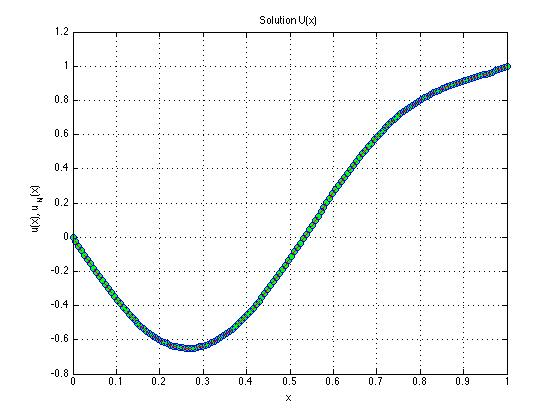
\includegraphics[width=\textwidth]{solutionk2.jpg}
%                 \caption{solution(k=2)}
%                 \label{fig:k2}
%         \end{subfigure}%
%         ~ %add desired spacing between images, e. g. ~, \quad, \qquad, \hfill etc.
%           %(or a blank line to force the subfigure onto a new line)
%         \begin{subfigure}[b]{0.45\textwidth}
%                 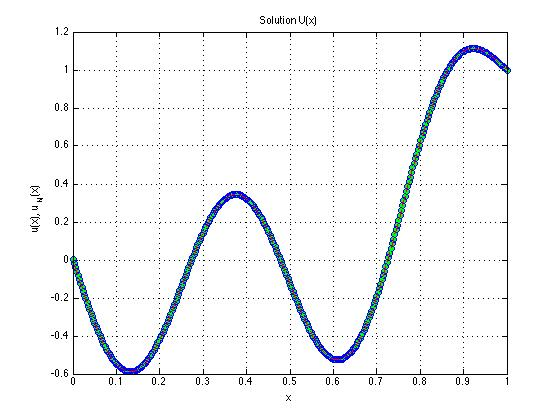
\includegraphics[width=\textwidth]{solutionk4.jpg}
%                 \caption{solution(k=4)}
%                 \label{fig:k4}
%         \end{subfigure}
%         %add desired spacing between images, e. g. ~, \quad, \qquad, \hfill etc.
%           %(or a blank line to force the subfigure onto a new line)
%         \begin{subfigure}[b]{0.45\textwidth}
%                 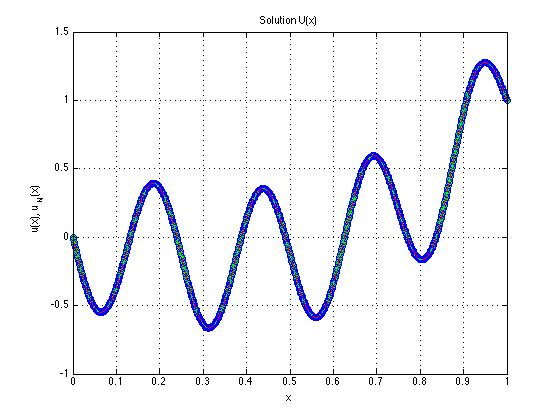
\includegraphics[width=\textwidth]{solutionk8.jpg}
%                 \caption{solution(k=8)}
%                 \label{fig:k8}
%         \end{subfigure}
%         ~ 
%          \begin{subfigure}[b]{0.45\textwidth}
%                 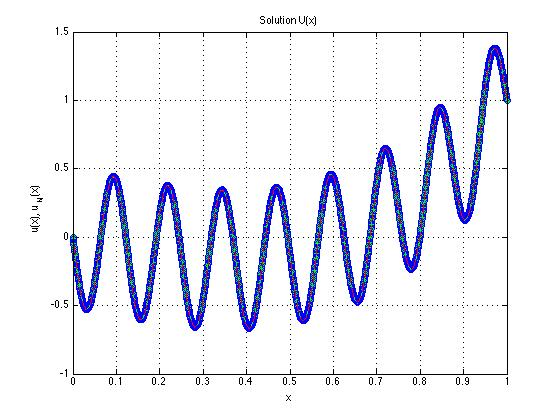
\includegraphics[width=\textwidth]{solutionk16.jpg}
%                 \caption{solution(k=16)}
%                 \label{fig:k8}
%         \end{subfigure}

%         \caption{solution u(x) and $u_N(x)$}\label{fig:solution}
% \end{figure}

% \begin{figure}
%         \centering
%         \begin{subfigure}[b]{0.45\textwidth}
%                 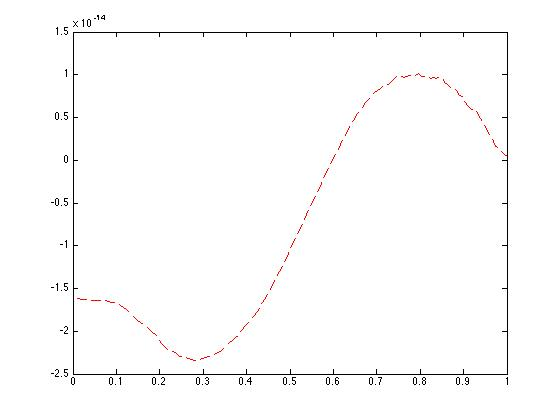
\includegraphics[width=\textwidth]{error2.jpg}
%                 \caption{error(k=2)}
%                 \label{fig:k2}
%         \end{subfigure}%
%         ~ %add desired spacing between images, e. g. ~, \quad, \qquad, \hfill etc.
%           %(or a blank line to force the subfigure onto a new line)
%         \begin{subfigure}[b]{0.45\textwidth}
%                 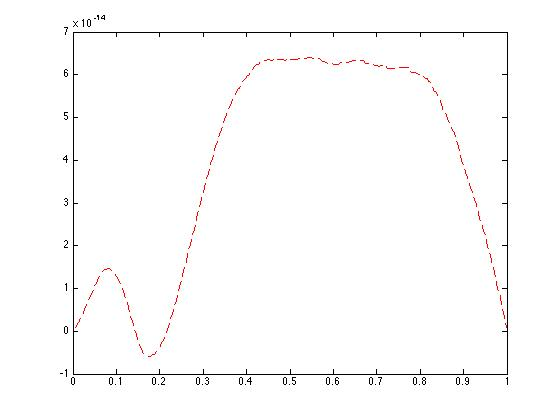
\includegraphics[width=\textwidth]{errork4.jpg}
%                 \caption{error(k=4)}
%                 \label{fig:k4}
%         \end{subfigure}
%         %add desired spacing between images, e. g. ~, \quad, \qquad, \hfill etc.
%           %(or a blank line to force the subfigure onto a new line)
%         \begin{subfigure}[b]{0.45\textwidth}
%                 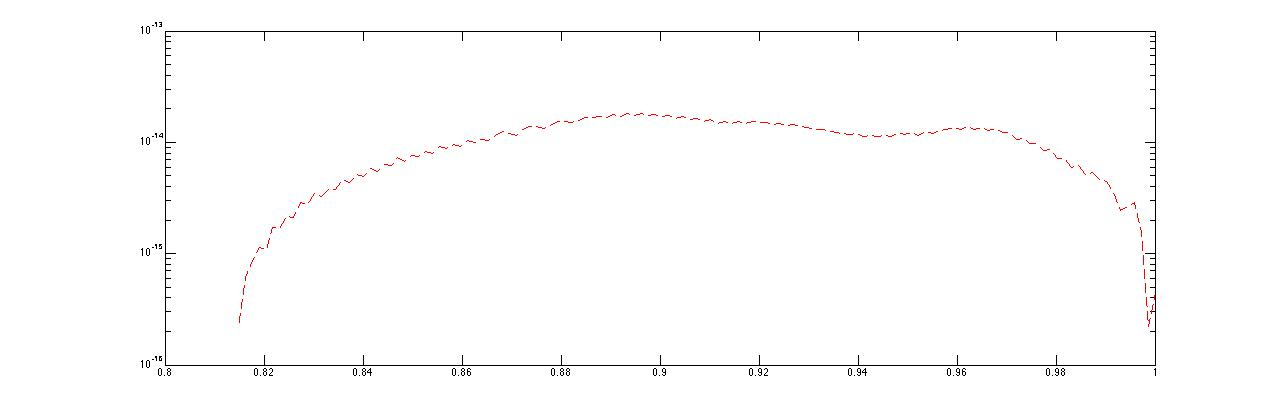
\includegraphics[width=\textwidth]{errork8.jpg}
%                 \caption{error(k=8)}
%                 \label{fig:k8}
%         \end{subfigure}
%         ~ 
%          \begin{subfigure}[b]{0.45\textwidth}
%                 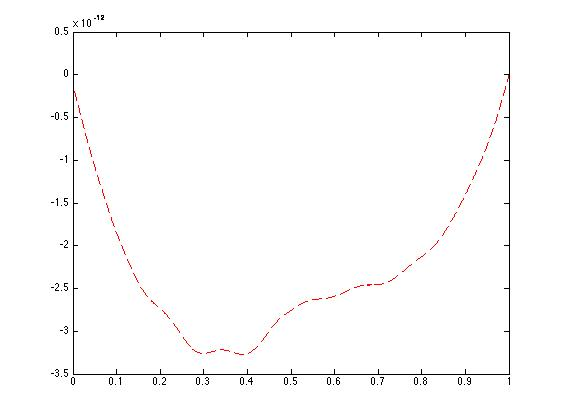
\includegraphics[width=\textwidth]{errork16.jpg}
%                 \caption{error(k=16)}
%                 \label{fig:k8}
%         \end{subfigure}

%         \caption{error between u(x) and $u_N(x)$}\label{fig:error}
% \end{figure}




\section{Conclusion}
With the constant k in the right side of the equation getting larger, the frequency of $sin(\pi k x /L)$ increases, so we need more nodes to capture the fluctuation of the solution. The number of elements needed for the same error criteria is almost proportional to k.

Three points gaussian quadriture is used in the project, giving exact integral values for polynomials with order 5 or less. 

Keeping in mind the computation cost is important for engineers. Several technics were used in this project to save the memory and computation cost, such as binary search and sparse matrix. 


\end{document}